\documentclass[unknownkeysallowed,usepdftitle=false]{beamer}
% unknownkeysallowed is needed for mac and the newer latex version -> is more picky than before...
%\usetheme[headheight=1cm,footheight=2cm]{boxes}
\usetheme[compress]{Cornell}
%\usetheme{Cornell}
%\usetheme{default}
%\input{config/commands}
\input{config/hyphenation}

\usepackage[utf8]{inputenc}
\usepackage{default}
\usepackage{graphicx}
\usepackage{epsfig}
\usepackage{siunitx}
\usepackage{color}
\usepackage{ifthen}
\usepackage{ragged2e}
\usepackage{mwe}
\usepackage{multicol}
\usepackage{tikz}
\usetikzlibrary{positioning}

\usepackage{bm}
\usepackage{amsfonts}
\usepackage{amssymb}

\setbeamertemplate{navigation symbols}{}%remove navigation symbols
%\setbeamersize{text margin left=0pt,text margin right=0pt}

% some colors
\definecolor{grau}{gray}{.5}
%\definecolor{slfcolor}{rgb}{0.698,0.847,0.796}
\definecolor{slfcolor}{rgb}{0.698,0.847,0.796}
\definecolor{titlecolor}{rgb}{0.489,0.593,0.557}
\definecolor{wslcolor}{rgb}{0,0.4,0.4}

\newcommand{\red}[1]{{\color[rgb]{1,0,0}#1}}
\def\colorize<#1>{\alt<#1>{\color{red}}{\color{black}}}


\newcommand{\tens}[1]{\mathbf{\mathrm{#1}}}
\renewcommand{\vec}[1]{\mathbf{#1}}
\renewcommand{\P}{\mathbb{P}}
\newcommand{\E}{\mathbb{E}}
\newcommand{\Exp}{\operatorname{Exp}}

% setup links
\hypersetup{%
	%linkbordercolor=green,%
	colorlinks=false,%
	pdfborderstyle={/S/U/W 0},%
	%pdfpagemode=FullScreen,%
	pdfstartpage=4%
	}

% setup some fonts
\setbeamerfont{title}{series=\bfseries, size=\small}
%\setbeamerfont{author}{size*={1pt}{0pt}}
\setbeamerfont{institute}{size*={3pt}{0pt}}
\setbeamerfont{bodytext}{size=\scriptsize}
	
% Title setup	
\title{
Reproducible %Open Source 
Carbon Cycle Models  \\  
Biogeochemical Model Database  \texttt{bgc\_md2}
}
\author{
\tiny Markus Müller, Holger Metzler, Verónika Ceballos Núñez, Kostiantyn Viatkin, Thomas Lotze, Jon Wells, Yu Zhou, Cuijuan Liao, Aneesh Chandel, Feng Tao, Yuanyuan Huang, Alison Bennett, Chenyu Bian, Lifen Jiang, Song Wang, Chengcheng Gang, Carlos Sierra, Yiqi Luo
 }
%\institute{Cornell University Ithaca NY}
\date{04-27-2023}
% add title in headbox
\setbeamertemplate{headline}
{\leavevmode
\begin{beamercolorbox}[width=1\paperwidth]{head title}
  \vspace{0.05cm}
  \begin{columns}[t, totalwidth=\textwidth]
  %\begin{column}[c]{.05cm}
  %  
\includegraphics[width=1cm]{bold_cornell_seal_cmyk_red}
  %\end{column}
  % TITLE
   \begin{column}[c]{0.55\textwidth}
   \centering \usebeamerfont{title} \textcolor{titlecolor}{\inserttitle} \\
    
\includegraphics[height=0.3cm, keepaspectratio]{bold_cornell_seal_cmyk_red}
    
\includegraphics[height=0.3cm, keepaspectratio]{minerva}
    
\includegraphics[height=0.3cm, keepaspectratio]{NAU}
    
\includegraphics[height=0.3cm, keepaspectratio]{idiv}
    \includegraphics[height=0.3cm, keepaspectratio]{Logo_of_the_University_of_Melbourne}
    
\includegraphics[height=0.3cm, keepaspectratio]{EastChinaUni.png}
    
\includegraphics[height=0.3cm, keepaspectratio]{IGSNRR}
    
\includegraphics[height=0.3cm, keepaspectratio]{Northwest_A&F_University}
    
\includegraphics[height=0.3cm, keepaspectratio]{SLU}
%   \vspace{-0.05cm}
%   \centering \usebeamerfont{institute} \insertinstitute
  \end{column}
  % PICUTRE
  \begin{column}[c]{0.45\textwidth}
    %\vspace{0.05cm}
    %\centering 
    %\usebeamerfont{author} 
    \color[rgb]{0,0,0} 
    {\tiny Markus Müller, Holger Metzler, Verónika Ceballos Núñez,
    Kostiantyn Viatkin, Thomas Lotze, Jon Wells, Yu Zhou, Cuijuan
    Liao, Aneesh Chandel, Feng Tao, Yuanyuan Huang, Alison Bennett,
    Chenyu Bian, Lifen Jiang, Song Wang, Chengcheng Gang, Carlos
    Sierra, Yiqi Luo
    }
  \end{column}
  \end{columns}
  {\color{white}\hrule height 1pt\vspace{0.1cm}}
\end{beamercolorbox}%
}

% setup the navigation in footbox
% first set some button colors
\newcommand{\buttonactive}{\setbeamercolor{button}{bg=wslcolor,fg=white}}
\newcommand{\buttonpassive}{\setbeamercolor{button}{bg=slfcolor,fg=black}}
% now set up that the one active one gets the new color.
\newcommand{\secvariable}{nothing}
% therefore we write before each section (well, everything which should be part of the navi bar)
% the variable \secvariable to any name which is in the next function ...
\newcommand{\mysection}[1]{\renewcommand{\secvariable}{#1}
}
% ... compaired to strings in the following navibar definition ...
\newcommand{\tocbuttoncolor}[1]{%
 \ifthenelse{\equal{\secvariable}{#1}}{%
    \buttonactive}{%
    \buttonpassive}
 }
% ... here we start to set up the navibar. each entry is calling first the function \tocbuttoncolor with the argument which should be tested for beeing active. if active, then change color. afterwards the button is draw. so to change that, you need to change the argument in \toc..color, the first in \hyperlink and before each frames definition... A bit messed up, but works...
\newlength{\buttonspacingfootline}
\setlength{\buttonspacingfootline}{-0.2cm}
\setbeamertemplate{footline}
{\leavevmode
\begin{beamercolorbox}[width=1\paperwidth]{head title}
  {\color{slfcolor}\hrule height 1pt}
  \vspace{0.05cm}
  % set up the buttons in an mbox
  \centering \mbox{
     \tocbuttoncolor{presentation}
     \hspace{\buttonspacingfootline}
       \hyperlink{presentation}{\beamerbutton{Presentation}}
     
     \tocbuttoncolor{Implementation}
     \hspace{\buttonspacingfootline}
       \hyperlink{implementation}{\beamerbutton{Implementation}}

     \tocbuttoncolor{screen shots}
     \hspace{\buttonspacingfootline}
       \hyperlink{screen_shots}{\beamerbutton{Screen Shots}}
     
     \tocbuttoncolor{Links}
     \hspace{\buttonspacingfootline}
       \hyperlink{links}{\beamerbutton{Links}}
%%     
%%     \tocbuttoncolor{maximum_entropy}
%%     \hspace{\buttonspacingfootline}
%%       \hyperlink{maximum_entropy}{\beamerbutton{Max. Entropy}}
%%
%%     \tocbuttoncolor{conclusions}
%%     \hspace{\buttonspacingfootline}
%%       \hyperlink{conclusions}{\beamerbutton{Conclusions}}
%%    
%%    \tocbuttoncolor{supplementary_material}
%%     \hspace{\buttonspacingfootline}
%%      \hyperlink{supplementary_material}{\beamerbutton{Suppl. Mat.}}
%     \tocbuttoncolor{minor}
%     \hspace{\buttonspacingfootline}
%       \hyperlink{minor}{\beamerbutton{Minor Surges}}
%     \tocbuttoncolor{friction}
%     \hspace{\buttonspacingfootline}
%       \hyperlink{friction}{\beamerbutton{Friction}}
%     \tocbuttoncolor{conclusion}
%     \hspace{\buttonspacingfootline}
%       \hyperlink{conclusion}{\beamerbutton{Conclusion}}

    % this last one should normaly not be used... it will open the preferences to change the 
    % behaviour of the acrobat reader in fullscreen -> usefull in pico...
    \setbeamercolor{button}{bg=white,fg=black}
    % for presentation
    %\hspace{-0.1cm}\Acrobatmenu{FullScreenPrefs}{\beamerbutton{\#}}
    % for upload
    
     
\Acrobatmenu{FullScreenPrefs}{\vspace{0.3cm}\hspace{0.24cm}\mbox{%
    \includegraphics[height=0.04\textheight,keepaspectratio]{%
	   CreativeCommons_Attribution_License}%
	  }}
   }
    \vspace{0.05cm}
\end{beamercolorbox}%
}

\newcommand{\shiftleft}[2]{\makebox[0pt][r]{\makebox[#1][l]{#2}}}

\setbeamertemplate{frametitle}
{%
\vspace{-0.165ex}

%\begin{beamercolorbox}[wd=\paperwidth,dp=1ex, ht=4.5ex, sep=0.5ex, colsep*=0pt]{frametitle}%
\begin{beamercolorbox}[wd=\paperwidth, ht=2.8ex ]{frametitle}%
    \usebeamerfont{frametitle}   \strut \insertframetitle  \hfill 
    \shiftleft{1.4cm}{
       % \raisebox{-0.6cm}[0pt][0pt]{
       %   
\includegraphics[height=1.4cm, keepaspectratio]{egu_ospp_label_blue}
       % }
    }
\end{beamercolorbox}%
}%

\begin{document}
%%%%%%%%%%%%%%%%%%%%%%%%%%%%%%%%%%%%%%%%%%%%%%%%%%%%%%%%%%%
\mysection{presentation}\label{presentation}

\begin{frame}\frametitle{How to find the right model for a job?}
  \begin{itemize}
   \item  We need Collections 
      \begin{itemize}
        \item   
          of {\bf models} e.g.: {\tiny 
            Arora2005GCB-1 ,CARDAMOM ,$\dots$, Zelenev2000MicrobialEcology 
          }
        \item of  {\bf properties} and diagnostics to {\bf compare} them by 
            
          \begin{itemize}
            \item   symbolic e.g. {\tiny mass balance, CompartmentalMatrix, InFluxes $\dots$}
            {\tiny
              \[
              \displaystyle
              \frac{d}{dt}\left[\begin{matrix}leaf\\wood\end{matrix}\right]
                =\left[\begin{matrix}I_{leaf}{\left(t
                \right)}\\I_{wood}\end{matrix}\right]+\left[\begin{matrix}-
                  k_{leaf 2 wood} - k_{leaf o}{\left(t \right)} &
                  k_{wood 2 leaf}\\k_{leaf 2 wood} & - k_{wood 2 leaf}
                  - k_{wood
                  o}\end{matrix}\right]\left[\begin{matrix}leaf\\wood\end{matrix}\right]
              \]
            }
          \item graphic, numeric e.g. {\tiny carbon flux diagrams, transit times, age distributions $\dots$}
            \begin{tabular}{lll}
              \raisebox{-.5\height}{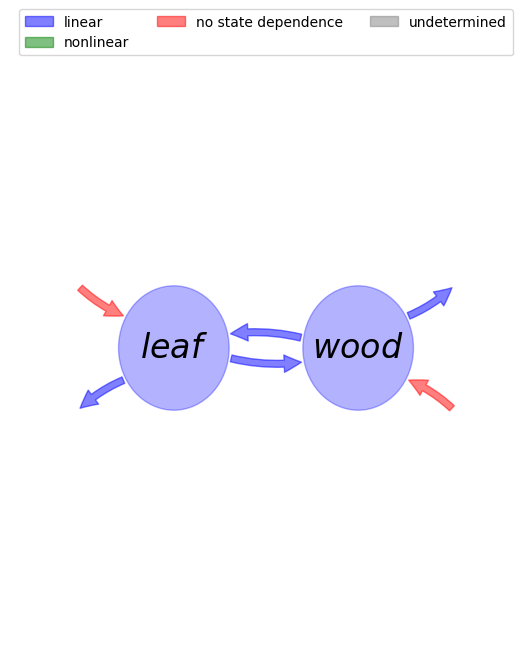
\includegraphics[height=2cm]{Figures/2pool}} 
              & 
              \raisebox{-.5\height}{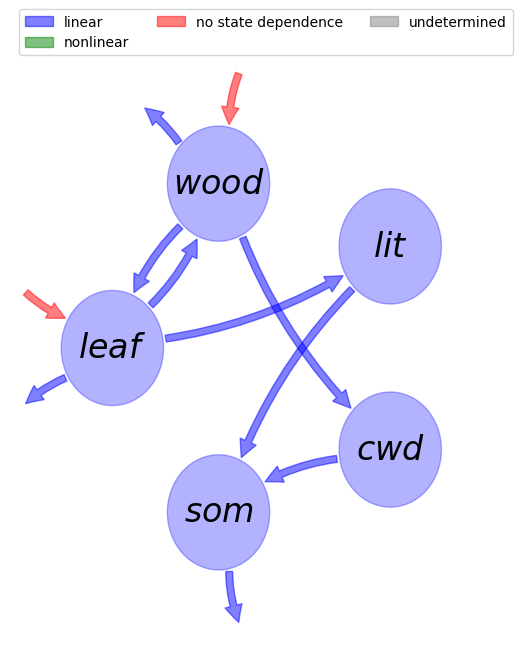
\includegraphics[height=2cm]{Figures/7pool}}
              & 
              \raisebox{-.5\height}{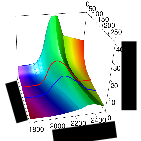
\includegraphics[height=2cm]{Figures/atmosphere_nonlinear}},
            %  & 
            %  $\dots$
            \end{tabular}
        \end{itemize}
      \end{itemize}
    \item {\bf HOW} do we implement, inspect, test and extend both collections? 
    \item {\bf HOW} can you steal from it?
  \end{itemize}
\end{frame}
     
%      \pause
%
%
%      How to formulate and run an element cycling model within a day?
%      \pause
%      \begin{tabular}{lll}
%        \raisebox{-.5\height}{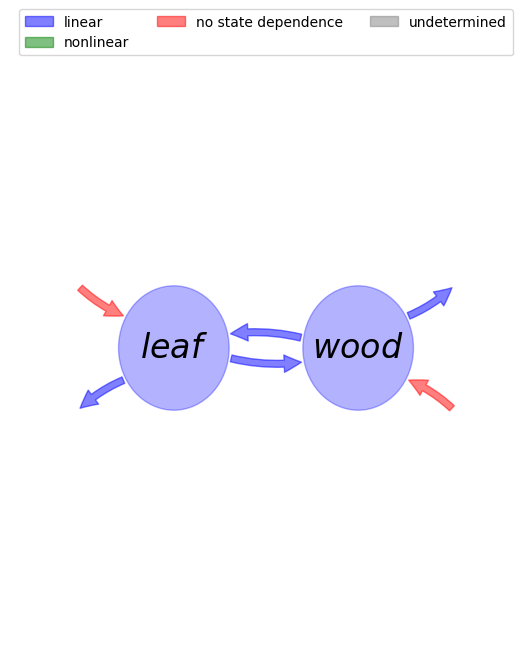
\includegraphics[height=2cm]{Figures/2pool}} 
%        & 
%        \begin{minipage}[c]{6cm}
%          \begin{itemize} 
%          \item 
%            test 
%          \end{itemize} 
%        \end{minipage}
%        & 
%        \raisebox{-.5\height}{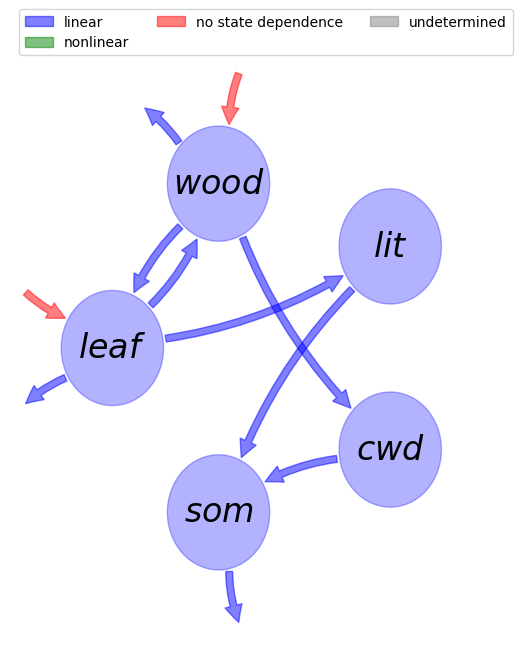
\includegraphics[height=2cm]{Figures/7pool}}
%        \\
%        simple 
%          & 
%          \centering{ 
%          $\rightarrow \dots \rightarrow \dots $ 
%          } 
%          & 
%          complex
%      \end{tabular}
%   \item  
%compare 
%      many models with respect to many different diagnostics reliably?
%   \item  
%How to allow models to be formulated in different ways?
%   \item  
%How to make runnable models transparent without implementation details obscuring the scientific content?
%   \item  
%How much does it cost? to keep the collection maintainable
%   \item  
%How to steal from the framework?     
%
%  \end{itemize}
%     

%%%%%%%%%%%%%%%%%%%%%%%%%%%%%%%%%%%%%%%%%%%%%%%%%%%%%%%%%%%
\mysection{Screen Shots}\label{screen_shots}
\subsection{Views}
\begin{frame}
\frametitle{Example widget for query result }
\centering{
	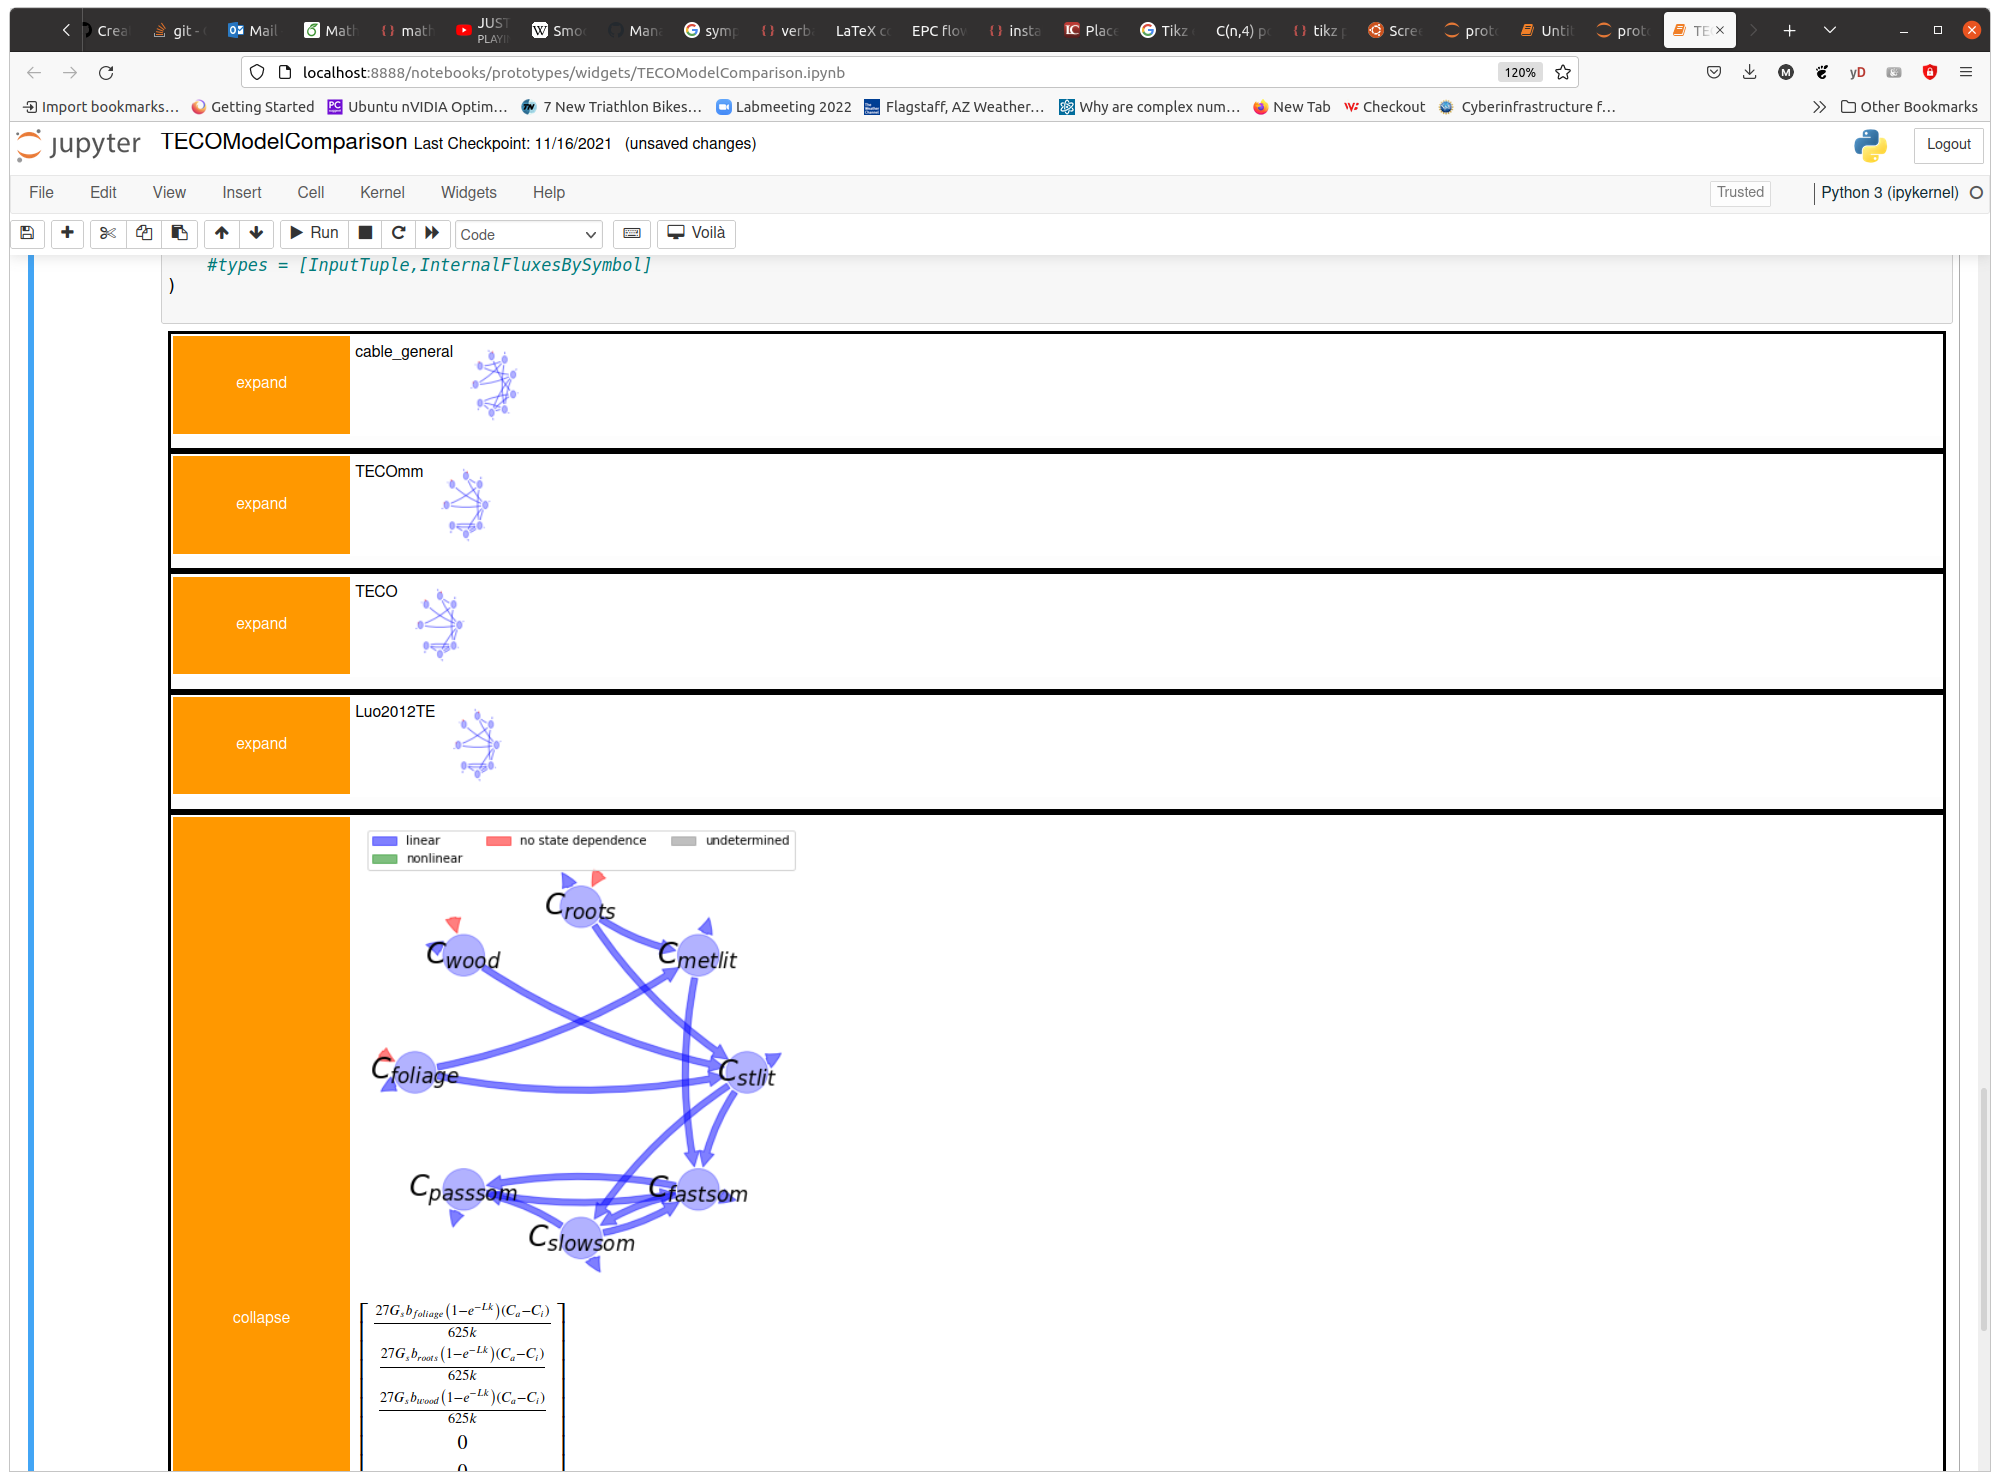
\includegraphics[height=.9\textheight]{ModelTable.png}
}
\note{
	\begin{enumerate}
	\item
	bgc\_md2 is an open source python package availabe on GitHub, developed at the Max-Planck-Institut for BioGeoChemistry in Jena and more recently  in Yiqi Luo's Ecolab at NAU in Flagstaff
	\item
	A set of libraries that can be used in other python scripts or interactively (jupyter or IPython )
	The picture shows a jupiter widget showing a table of models. The orange buttons can be clicked to 
	expand or collape a more detailed view of the particular model.
	\item
	$>$ 30 published vegetation, soil or ecosystems models in a format that
	for symbolic and numeric computations
	\item
	A set of special datatypes that describe components of the models and functions that operate on these datatypes
	\item 
	A userinterface that uses a graph library to compute what is computable and can be used for comparisons.
	\end{enumerate}
}
\end{frame}

\subsection{Single Model Inspection}
\begin{frame}
	\frametitle{Analysis with symbolic tools \dots}
  \centering{
	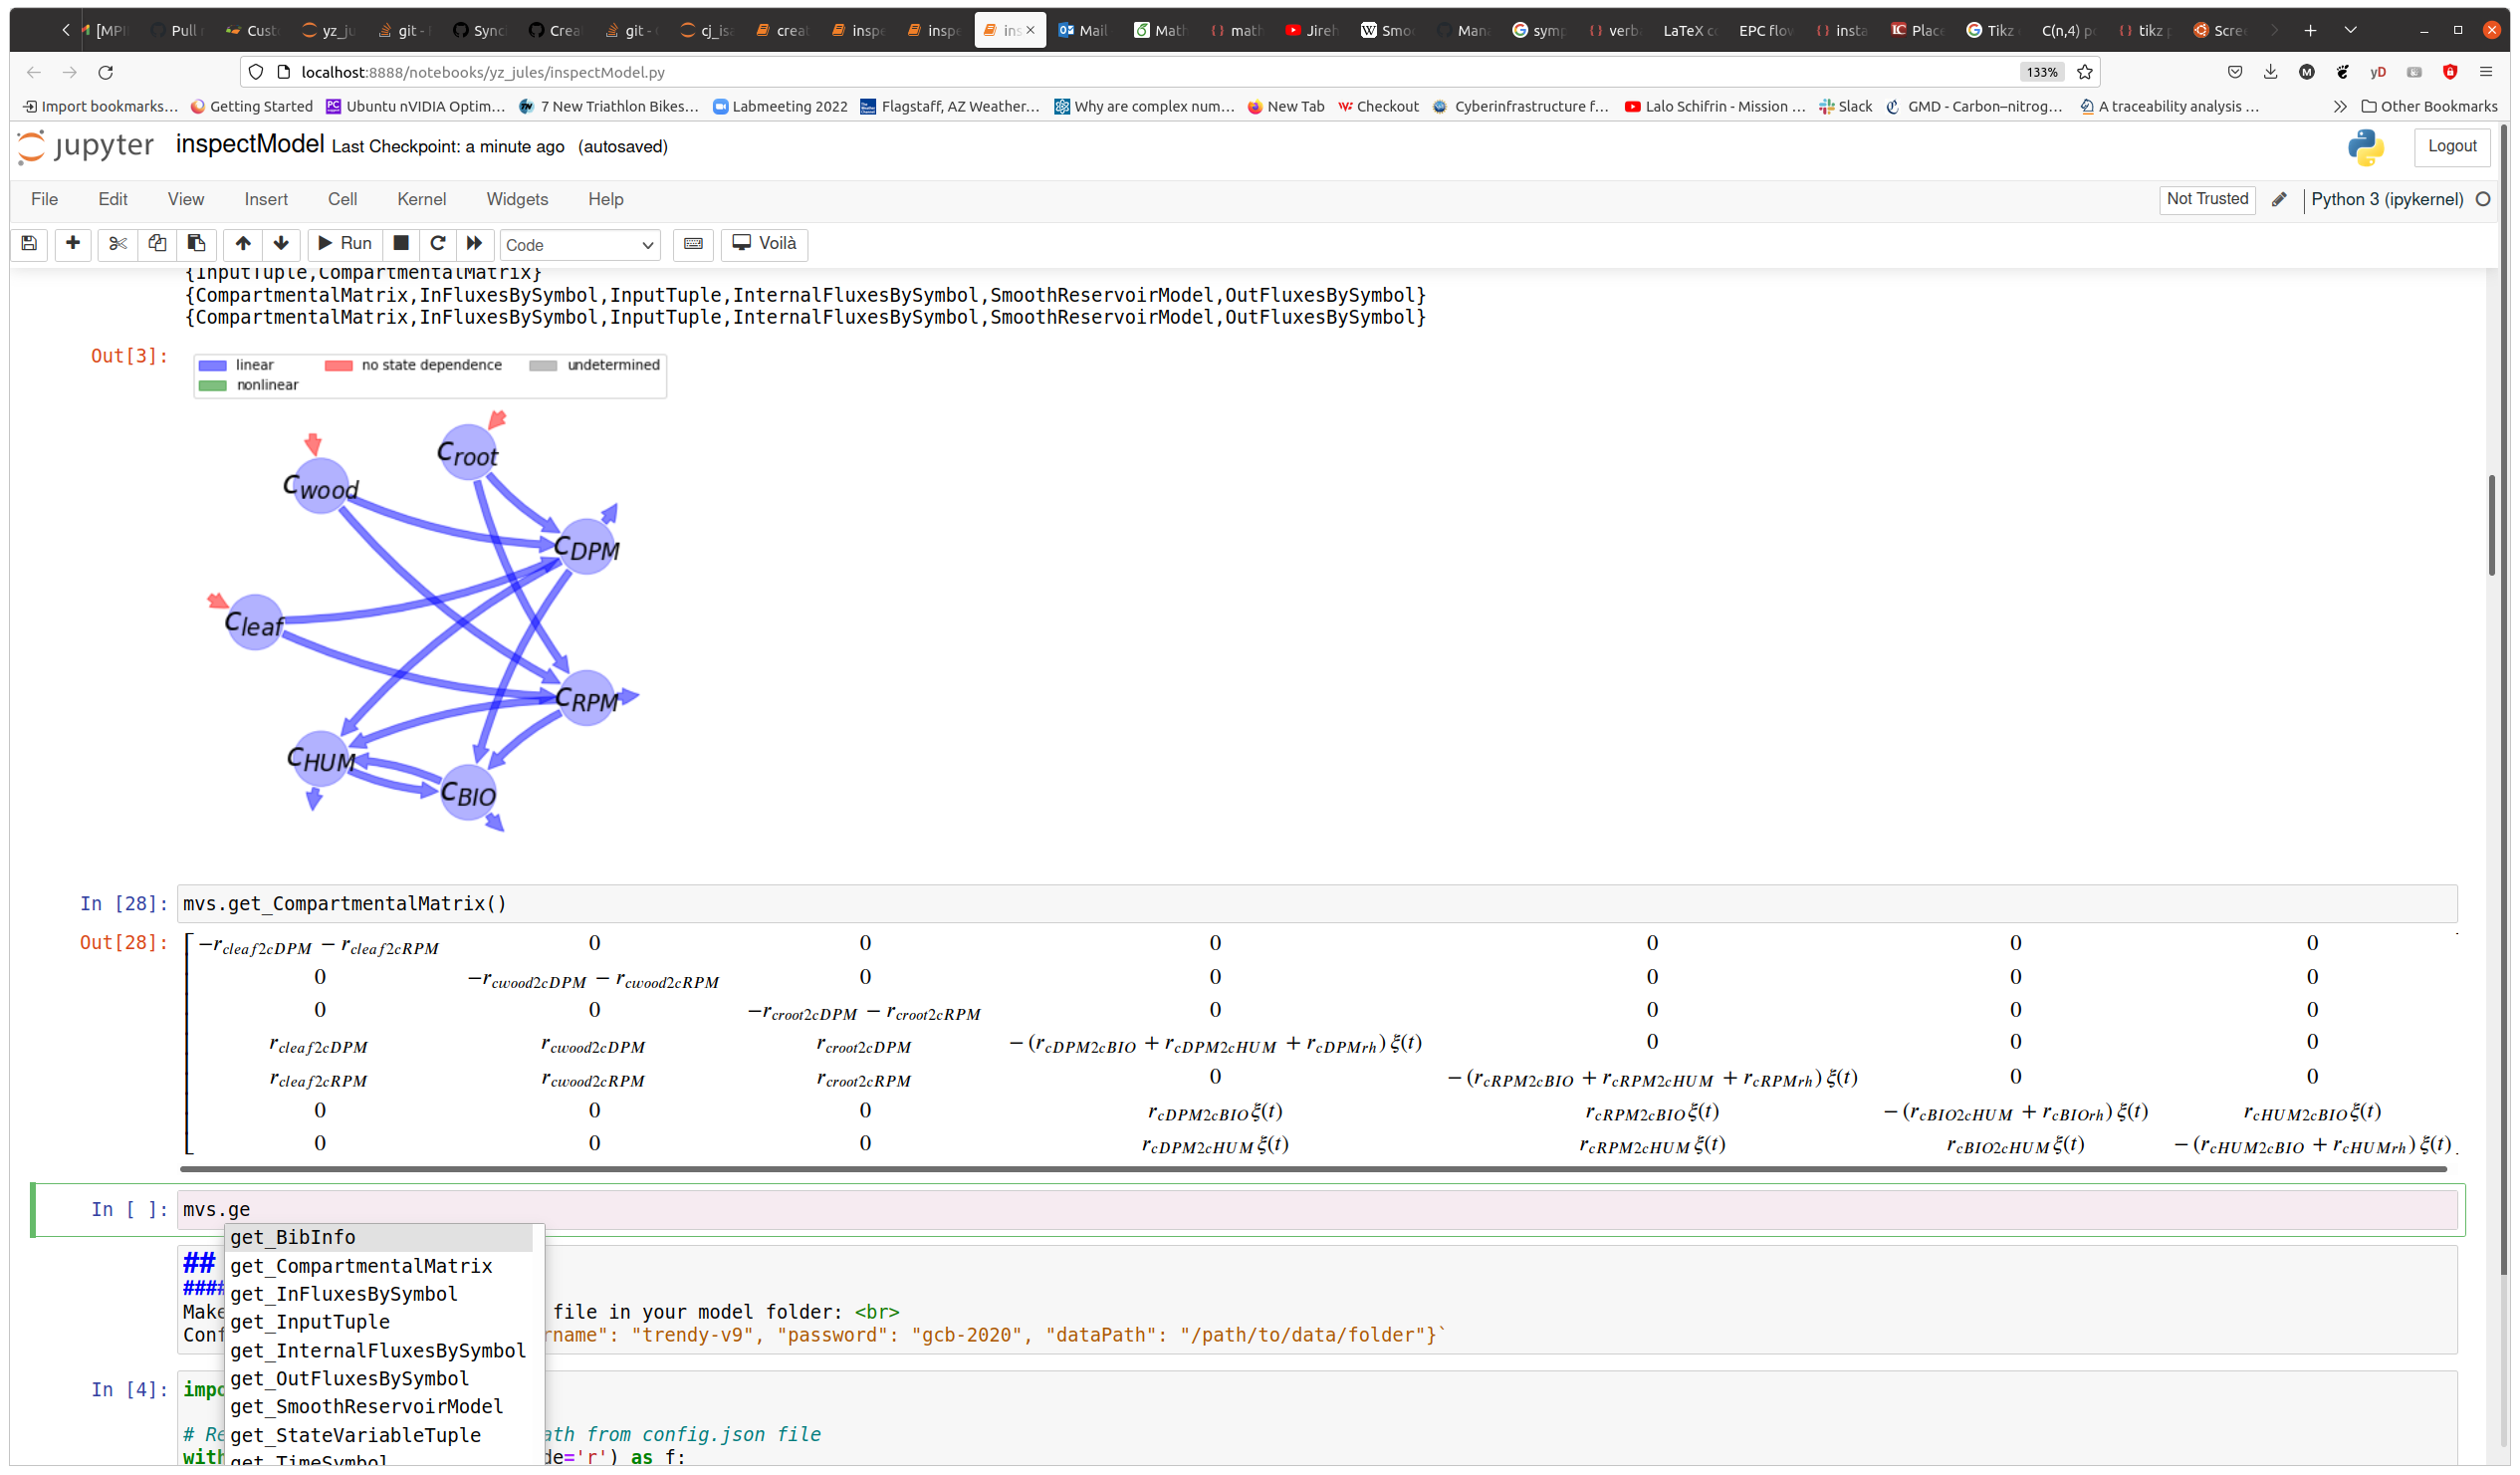
\includegraphics[height=.9\textheight]{mvsTabScreen.png}
  }
	\note{
	\begin{enumerate}
	\item 
	the structure (graph both in the mathematical and visual sense) can be derived from the symbolic description
	\item other properties are flux equations the compartmental matrix

	\end{enumerate}
	}
\end{frame}

\begin{frame}
	\frametitle{\dots or numerically }
  \centering{
	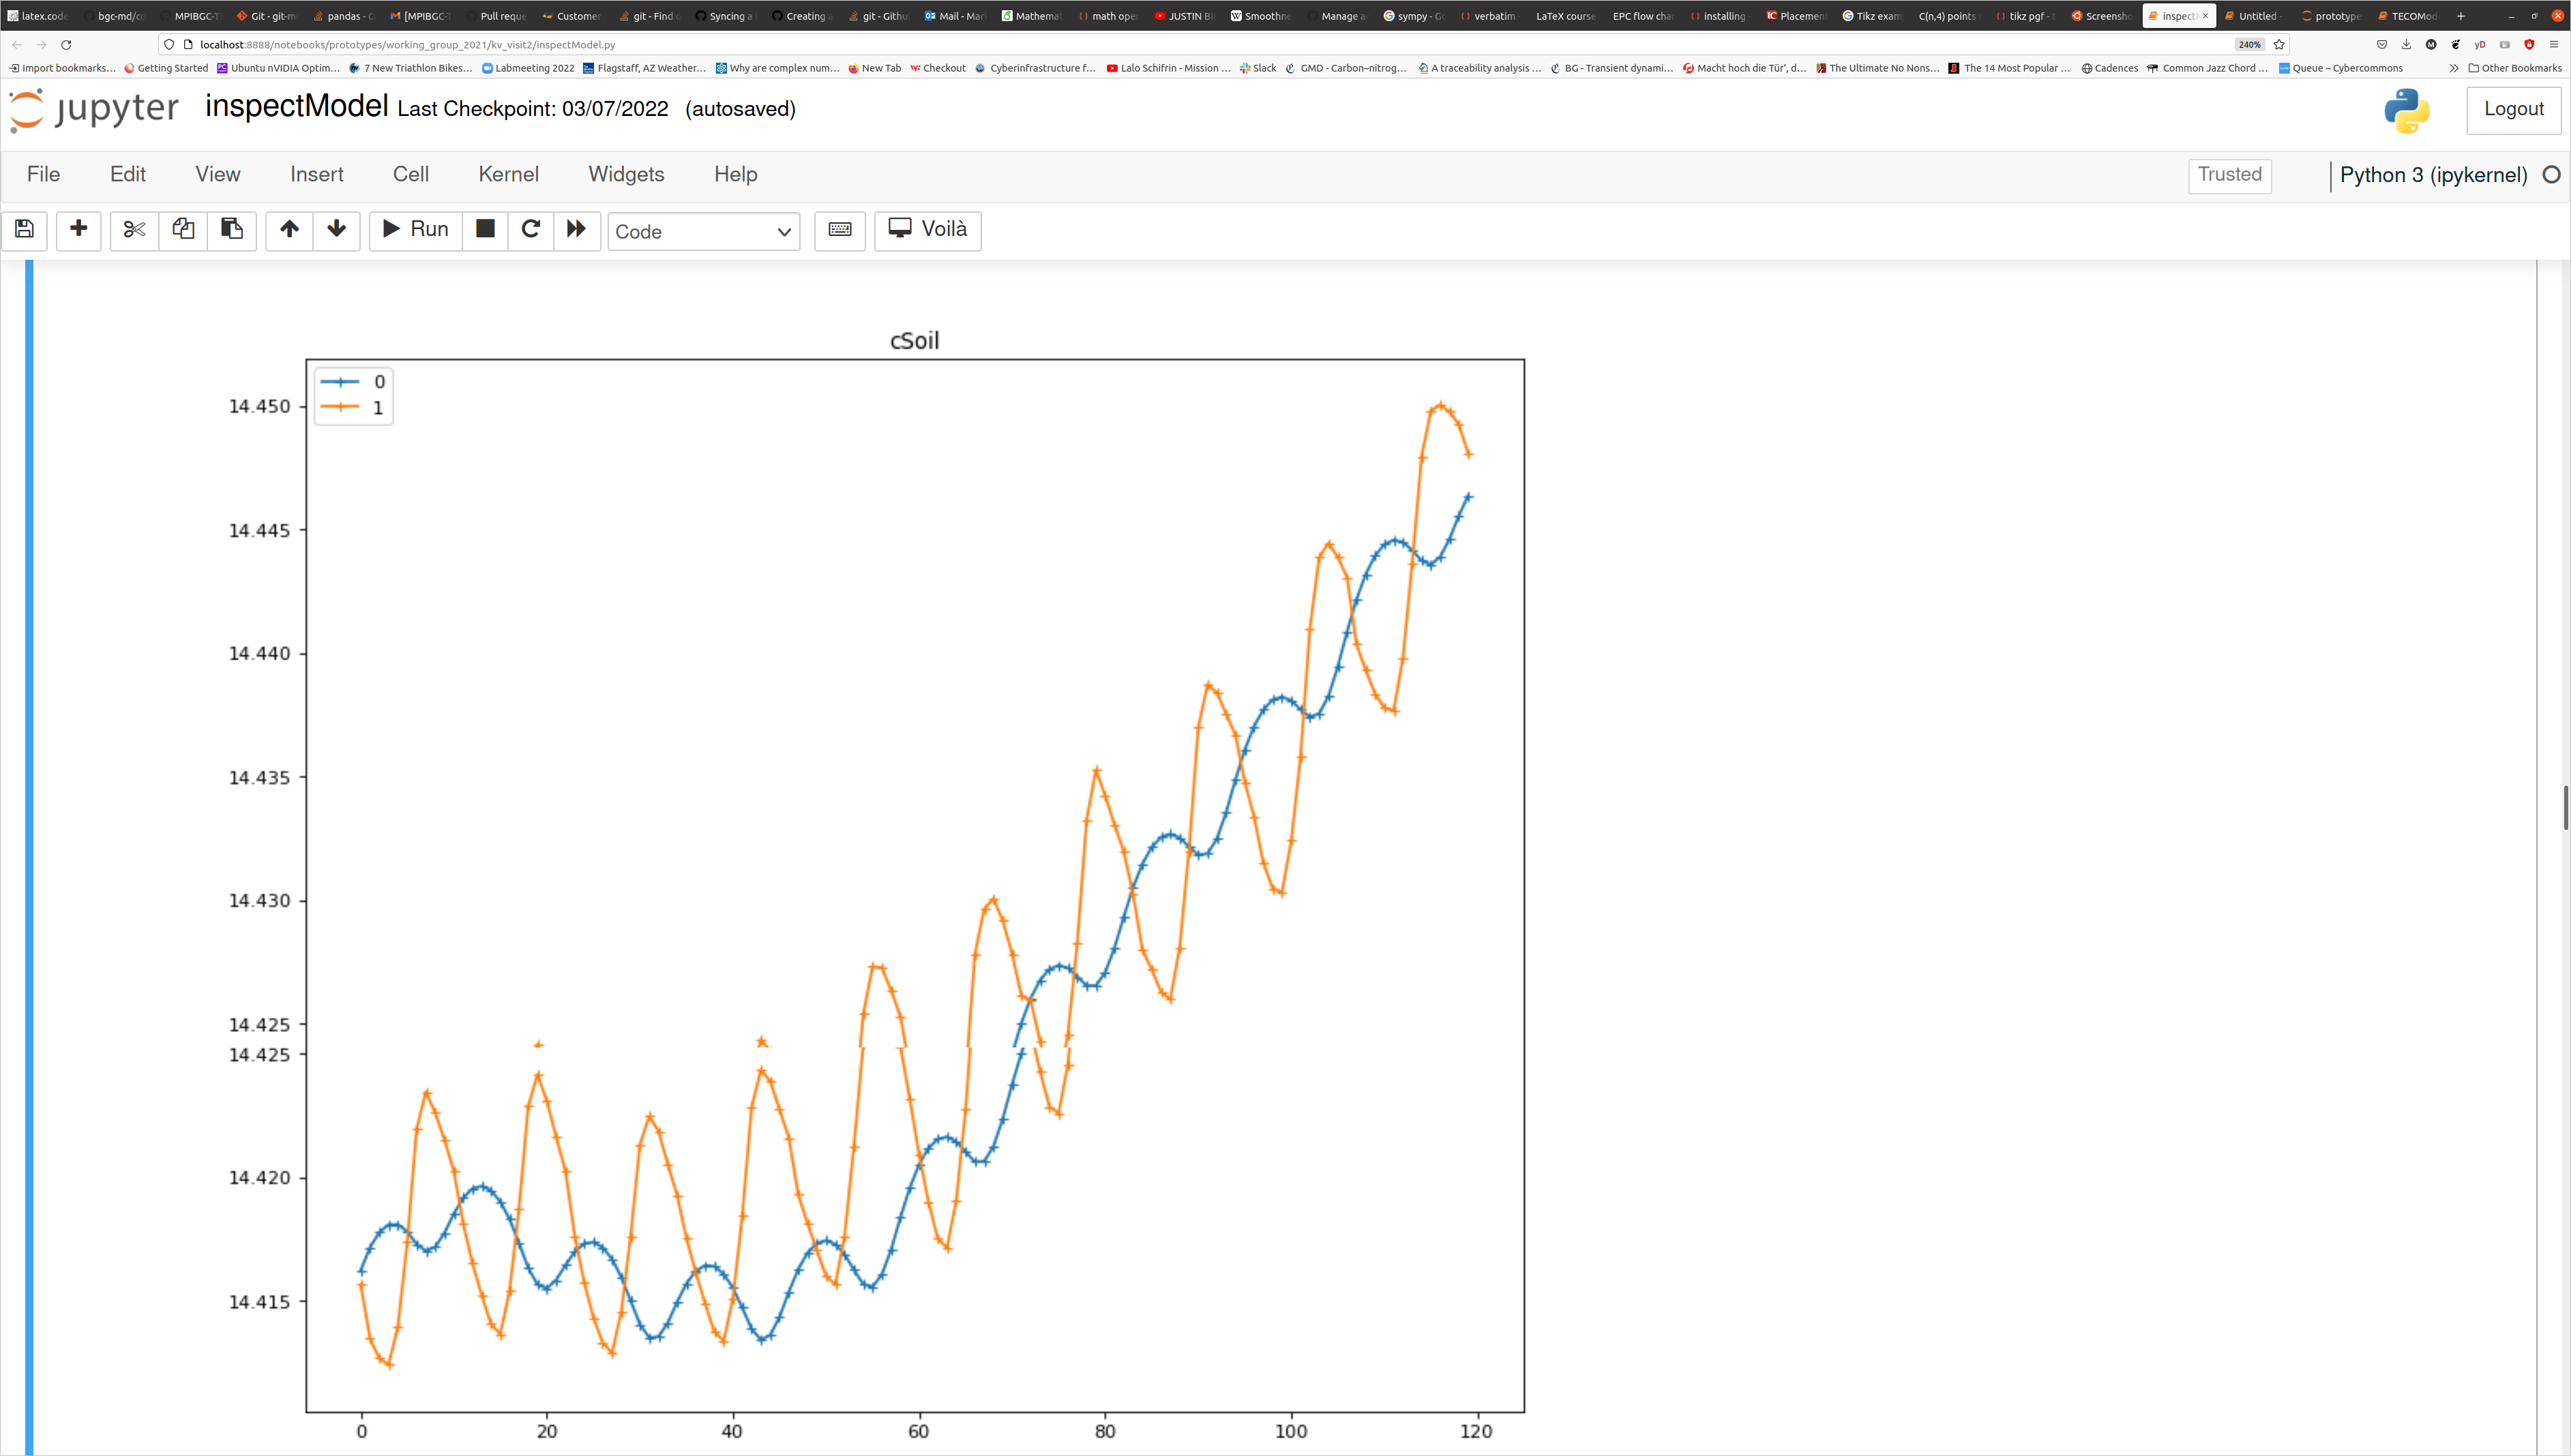
\includegraphics[height=.9\textheight]{DataAssimilation.png}
  }
	\note{
	\begin{enumerate}
	\item 
	the symbolic model description can be parameterized and transformed into a numeric model
	\item The picture shows the data assimilation result for the above model using trendy data.

	\end{enumerate}
	}
\end{frame}

%%%%%%%%%%%%%%%%%%%%%%%%%%%%%%%%%%%%%%%%%%%%%%%%%%%%%%%%%%%%
%\begin{frame}
%	\frametitle{Implemented diagnostics are available for all models}
%	\begin{figure}
%  \centering{
%	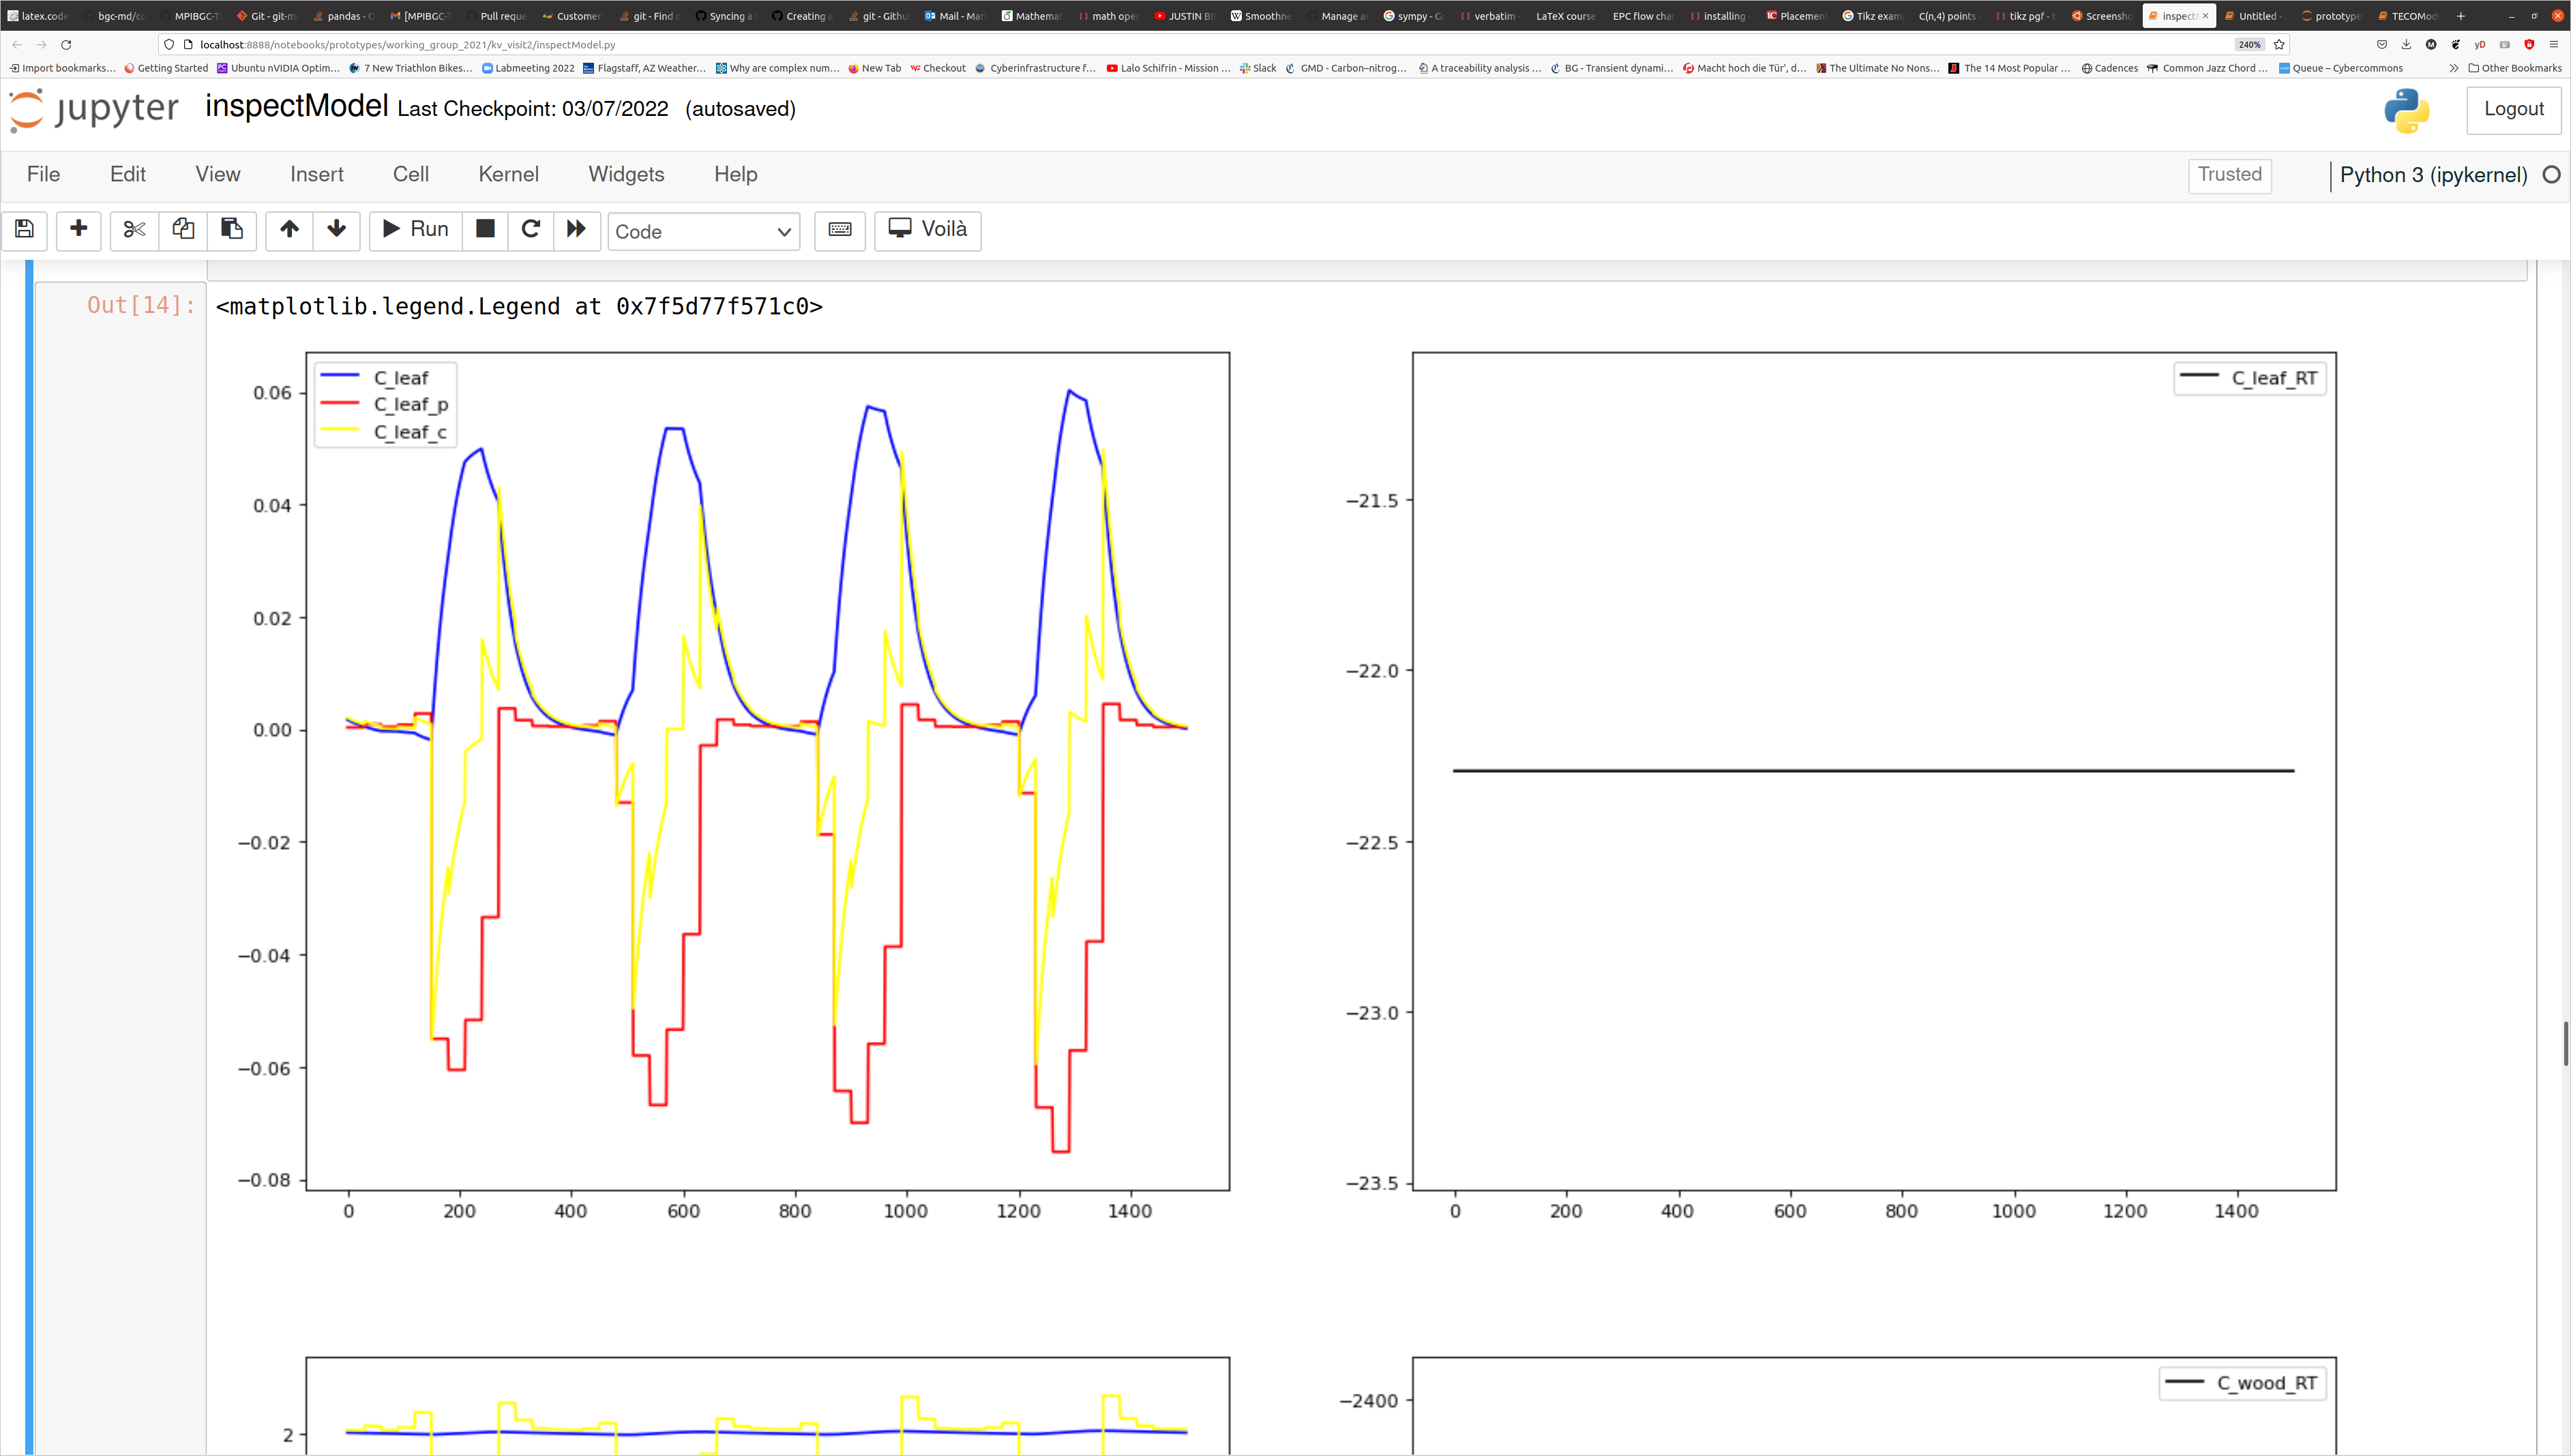
\includegraphics[height=.9\textheight]{TracebilityAnalysis.png}
%  }
%	\caption{pool content + Tracebility Analysis: carbon storage potential , carbon storage capacity and residence time}
%	\end{figure}
%	\note{
%	\begin{enumerate}
%	\item 
%	Diagnostic Variables can be computed for any model  
%	\item The picture shows the Leaf pool
%
%	\end{enumerate}
%	}
%\end{frame}
%%%%%%%%%%%%%%%%%%%%%%%%%%%%%%%%%%%%%%%%%%%%%%%%%%%%%%%%%%%
\mysection{Implementation}\label{implementation}
\subsection{A Record}
\begin{frame}
\frametitle{Database records are python modules}
  \centering{
  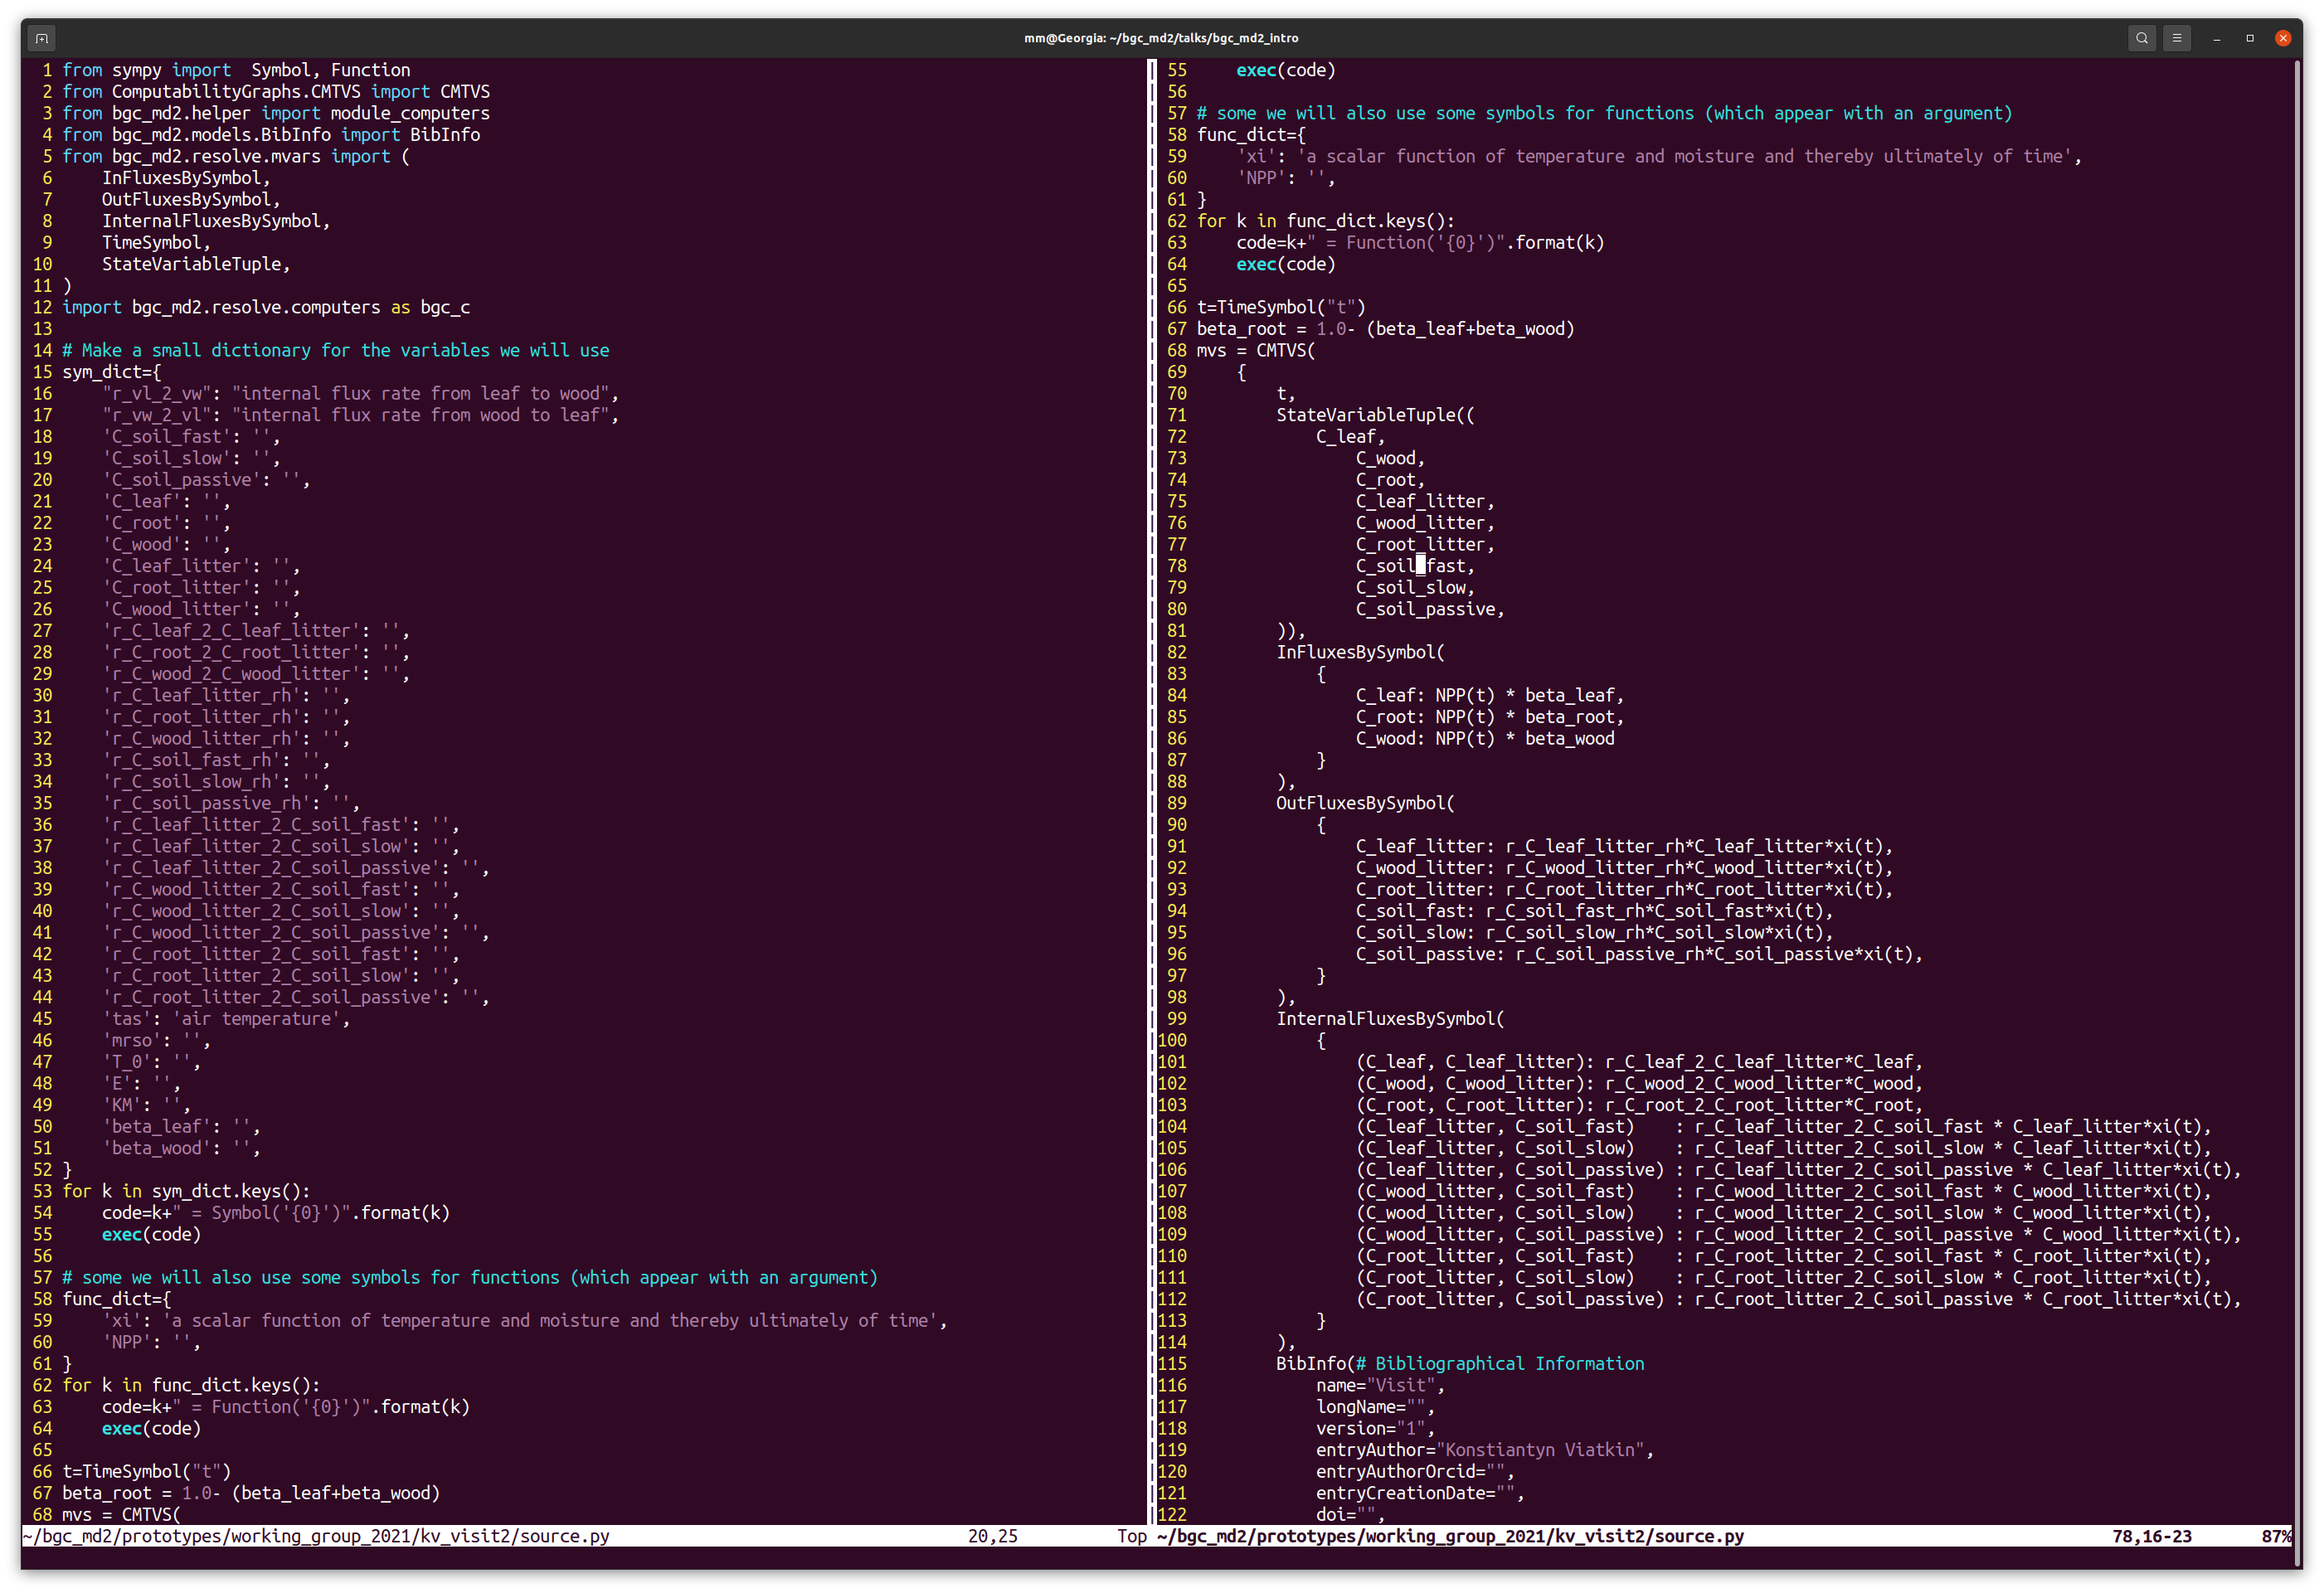
\includegraphics[height=.9\textheight]{source.py.png}
  }
  \note{
  \begin{enumerate}
    \item
    The picture shows the screen shot of the source code of the above model using sympy and some datatypes provided by \texttt{bgc\_md2}  .
    \item
    The entries of the database dont even have to be complete models. They are implemented in normal python and 
    have in common that they define a set of model properties and a set of functions to connect them.
    There is no special format necessary. 
    The creation of the symbolic formulation can be automated by all means available in python.
    Extra information can but does not have to be provided.
  \end{enumerate}
}
\end{frame}

%%%%%%%%%%%%%%%%%%%%%%%%%%%%%%%%%%%%%%%%%%%%%%%%%%%%%%%%%%%
\subsection{Classes \emph{and} Functions}
\begin{frame}
\frametitle{Internal Structure of \texttt{bgc\_md2}}
  \centering{
  \begin{tikzpicture}[sibling distance=12em,
    every node/.style = {shape=rectangle, rounded corners,
      draw, align=center,
      top color=white, bottom color=blue!20}]]
    \tikzstyle{level 1}=[sibling distance=14em]
    \tikzstyle{level 2}=[sibling distance=5em]
    \tikzstyle{level 3}=[sibling distance=3em]
    \tikzstyle{level 4}=[sibling distance=1.75em]
      \node {% <- this 'right of' is inherited; how to avoid?
      \begin{tikzpicture}[anchor=center]
        \node {\texttt{bgc\_md2}
        %\draw (0,0) -- (0,1);
        %\node[fill] at (0,.5) {};
        } 
        child{ node {models}
  	 child{ node{rothC}
  	    child{node {Fluxes}}
  	    child{node {Pools}}
  	    child{node {\dots}}
  	}
        	child{ node {Wang}
  	%    child{node {Fluxes}}
  	%    child{node {Pools}}
  	%    child{node {\dots}}
  	}
        	child{ node {\dots}}
        }
        child{ node {computers}
  	 child{node {Matrix(Fluxes)}}
  	 %child{node {Fluxes(Matrix,Pools)}}
  	 child{node {\dots}}
        };
      \end{tikzpicture}
      };
  \end{tikzpicture}
}
\note{
  \begin{enumerate}
    \item
    \texttt{bgc\_md2} is not just a collection of models, described as sets of varible of special type like fluxes or matrice, but also 
    a collection of functions whose arguments and return values have these types.
    These functions are here called \texttt{computers} and use python type annotations.
    The computability graph used in the user interface and queries is derived from the 
    annotations of a set of functions.
    The set of properties (defined by the types) is growing as well as the functions connecting them.
  \end{enumerate}
}
\end{frame}
%%%%%%%%%%%%%%%%%%%%%%%%%%%%%%%%%%%%%%%%%%%%%%%%%%%%%%%%%%%%%%%%%%%%%%%%%
\begin{frame}
  \frametitle{The \texttt{bgc\_md} library provides I:}
  
  \begin{enumerate}
    \item
      Datatypes defining building blocks of models e.g.\ \texttt{CompartmentalMatrix}, \texttt{InternalFluxesBySymbol}, \dots     
    \item
      Functions operating on those properties (forming the edges of the graph where the Datatypes are nodes) 
    \item
      A user interface based on graph algorithms to  
    \begin{enumerate}
      \item
        compute the set of computable properties (e.g. the comparable criteria for a set of models, database queries ) 
      \item
        actually compute the desired properties by recursively connecting several function applications.
      \item
        show what is missing to compute a desired property.
    \end{enumerate}
  \end{enumerate}
\end{frame}
%%%%%%%%%%%%%%%%%%%%%%%%%%%%%%%%%%%%%%%%%%%%%%%%%%%%%%%%%%%%%%%%%%%%%%%%%%%%
\subsection{Invisible Graphs}
\begin{frame}
  \frametitle{Userinterface using computability graphs}
  \centering{
  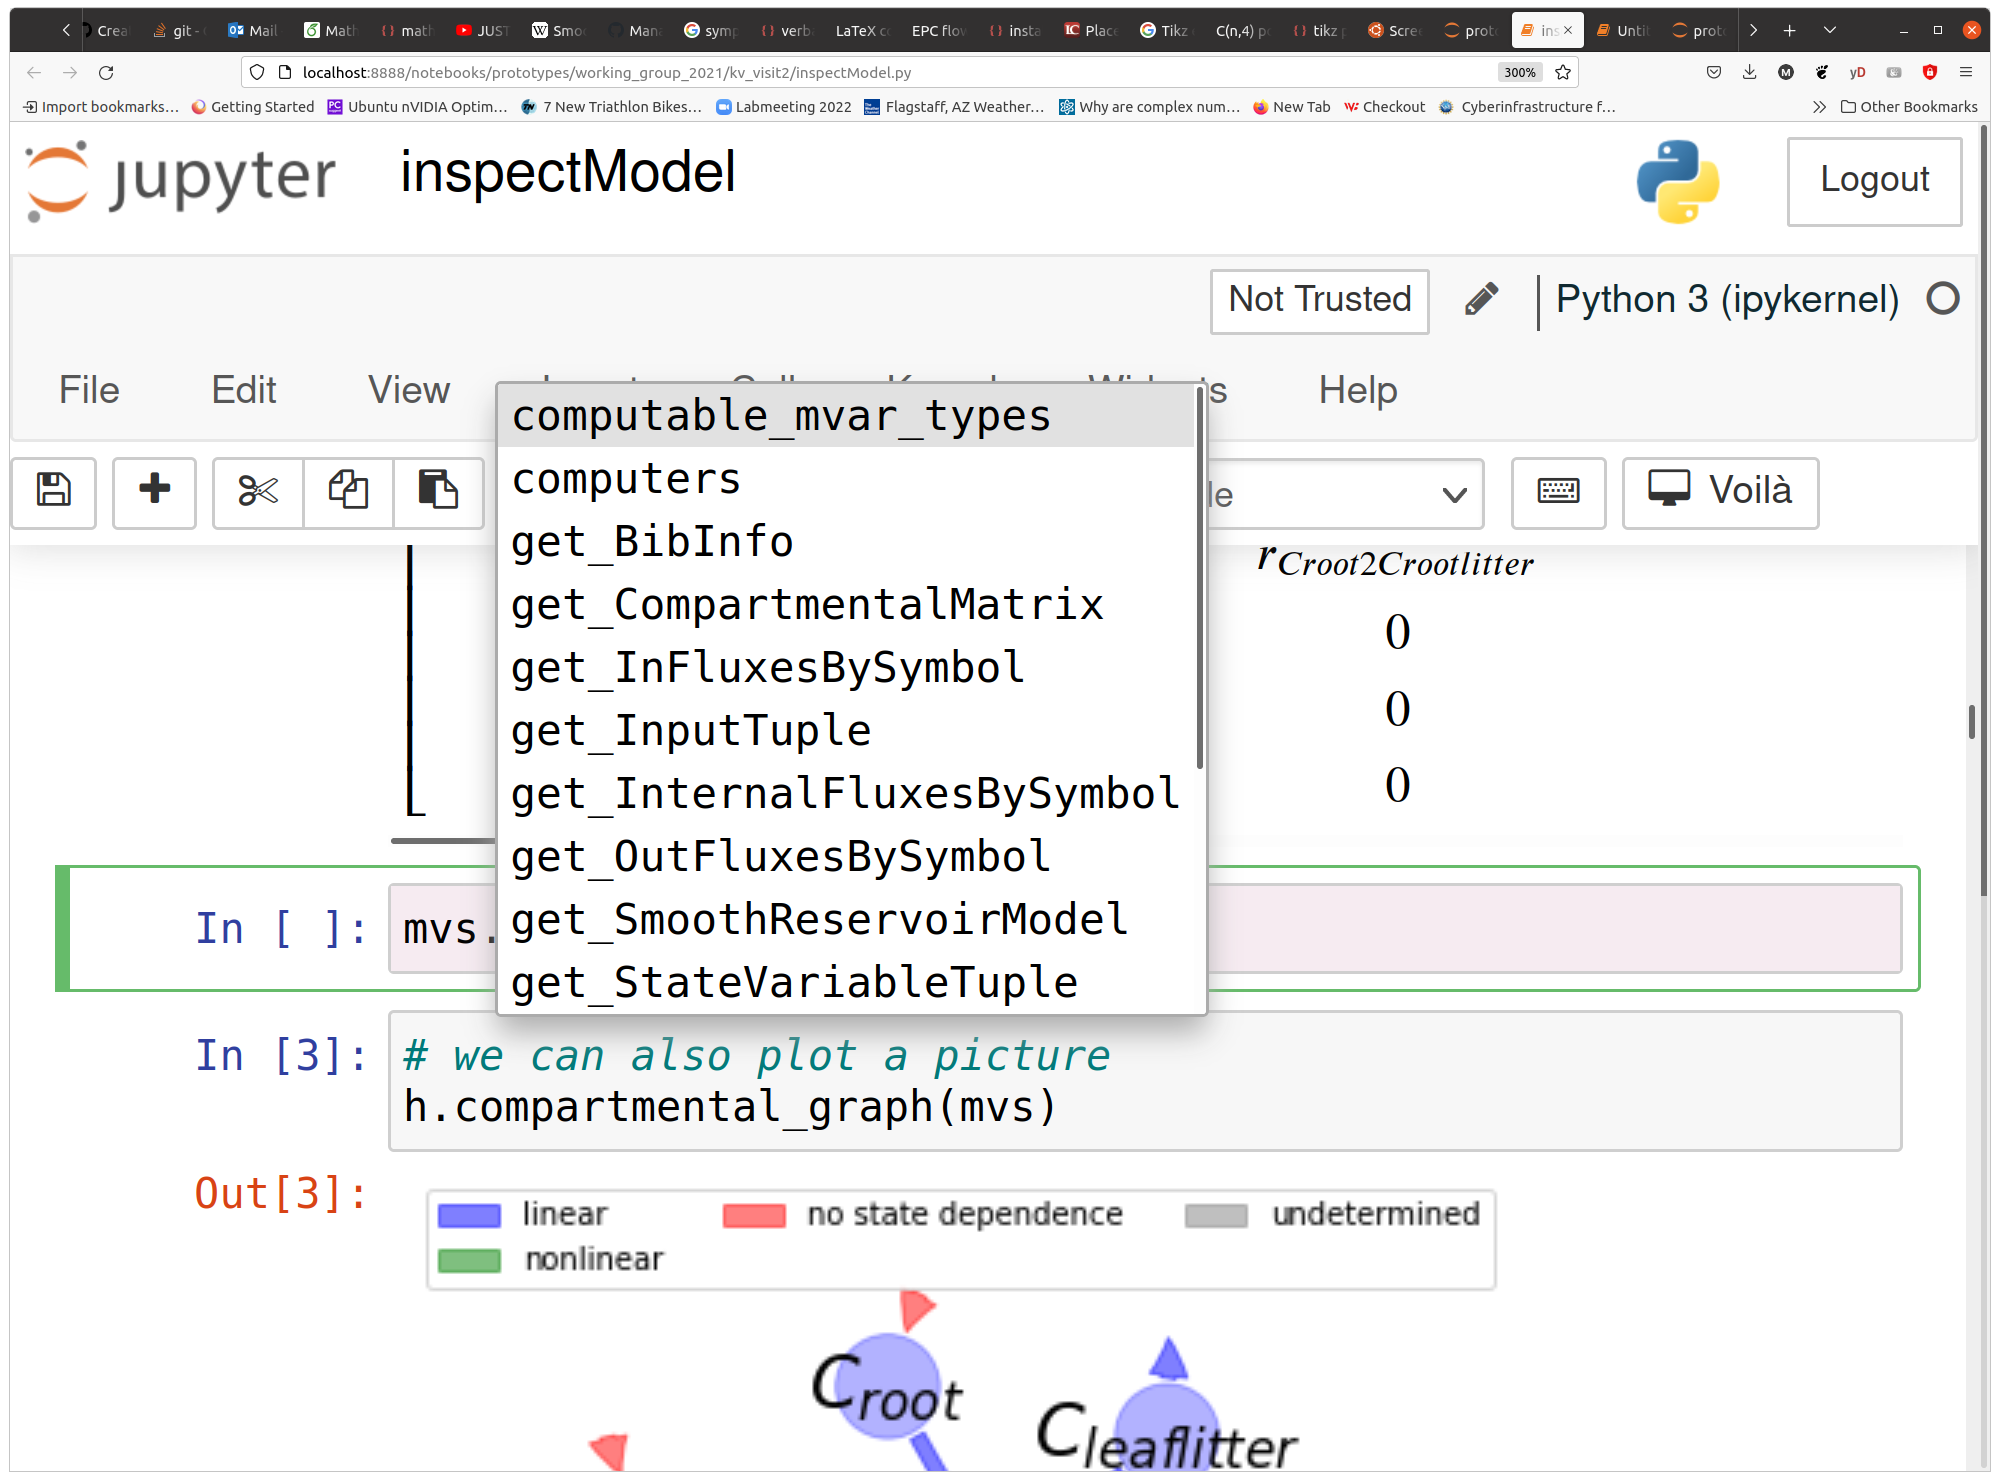
\includegraphics[height=0.7\textheight]{mvsTabScreenBig.png}
  \\
  Suggested methods automatically created by a graph library
  }
  \note{
  \begin{tiny}
    \begin{enumerate}
    \item
    The figure shows IPythons options for callable methods on a variable called \texttt{mvs} 
    \item
    This is standard for mehtods of a python object. 
    In this case the methods are automatically created and added by a graphalgorithm that computes 
    which variables can be computed form the set of provided model properties.
    \item 
    This has far reaching consequences.
    Models can be compared with respect to all variables in the "convex hull under computability', 
    with respect to all \emph{computable variables} not just the ones provided in the data base record.
    \item
    As an example the matrix formulation of models A and B  can be compared even if neither A nor B defines
    the matrix as long as it can be computed from other variable (in this case the internal and outfluxes and an ordering of the statevariables)
    \item
    An obvious consequence is that the information about a model can be provided in different ways.
    There is no need to force the user into a rigid record format.
    Another consequence is that records do not have to be complete. The framework accepts all information
    about a model and (computes what it can do with it).
    \item
    The set of computable properties can be used to query the database (e.g. which models have a vegetation part)
    \dots
    \end{enumerate}
  \end{tiny}
  }
\end{frame}
%%%%%%%%%%%%%%%%%%%%%%%%%%%%%%%%%%%%%%%%%%%%%%%%%%%%%%%%%%%%%%%%%%%
\subsection{Making them Visible }
\begin{frame}
  \frametitle{Finding what's missing in the model description }
\begin{columns}
  \begin{column}{0.3\textwidth}
  given a set of functions:\\
        a(i), b(c,d), b(e,f), c(b),
        d(b), d(g,h),
        e(b),
        f(b)
  and the target variable {\color{red}B}
  e.g. \texttt{CompartmentalMatrix},
  The algorithm computes all possible combinations
  and paths from which {\color{red}B} can be computed.
  \end{column}
  \begin{column}{0.7\textwidth}
      \begin{center}
      \begin{figure}
  	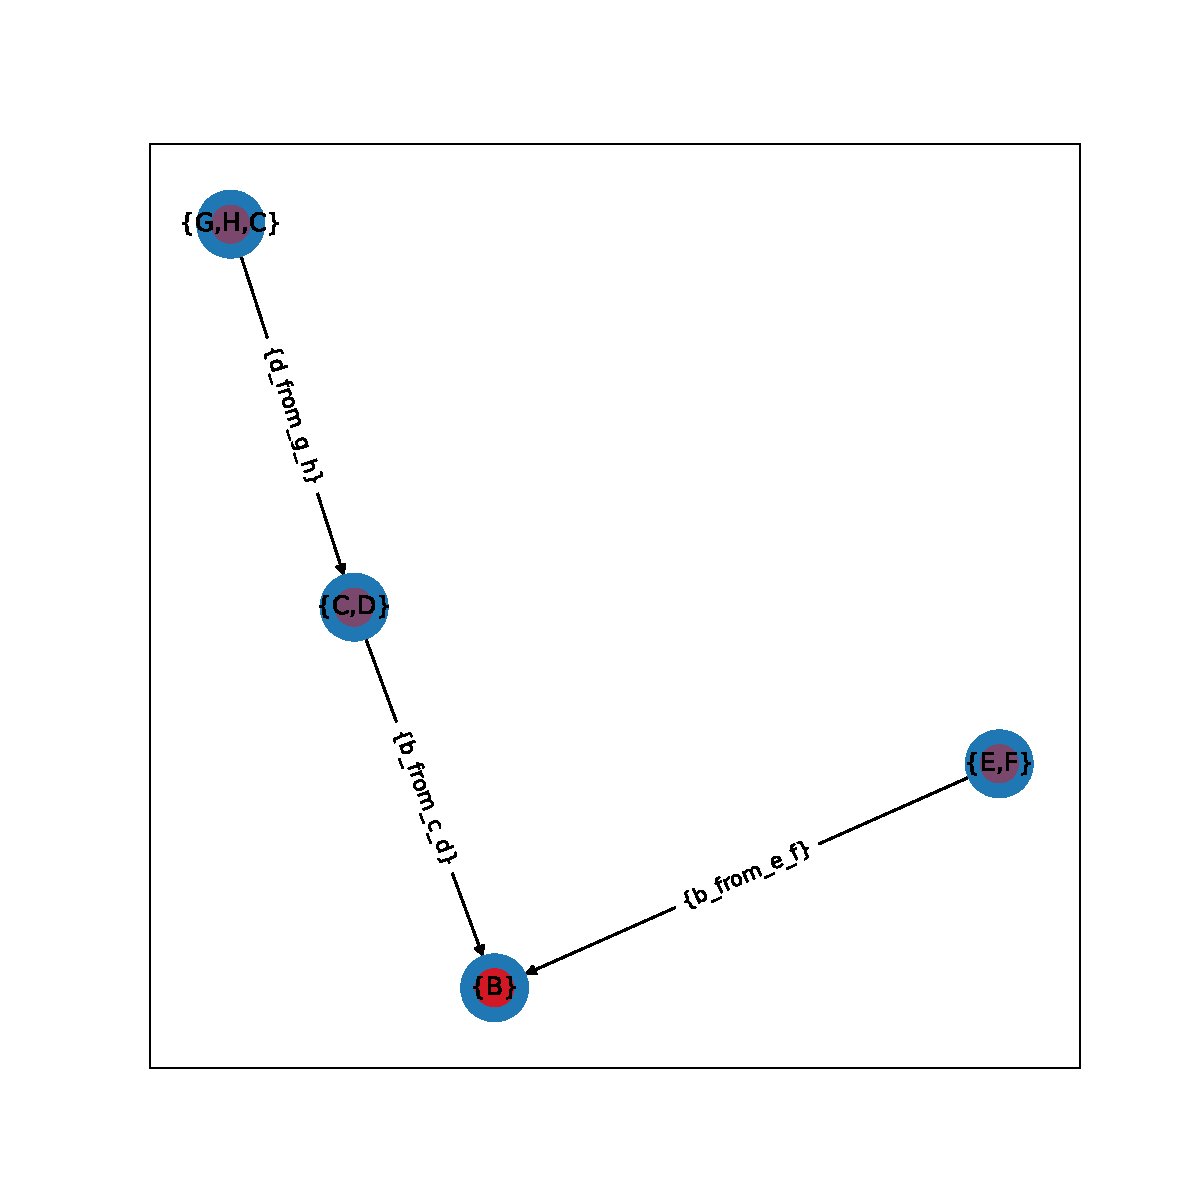
\includegraphics[height=.9\textheight]{StartNodes.pdf}
	%\caption{The computability Graph for variable B (e.g. \texttt{CompartmentalMatrix}}
      \end{figure}
       \end{center}
  \end{column}
\end{columns}
  \note{
    \begin{enumerate}
    \item
    It is not only possible to compute what can be computed from a given model description,
    It is also possible to do the opposite and ask the algorithm what missing information has to be 
    provided to compute a target property of a  model.
    \item
    The algorithm finds a path (a combination of functions that can be applied recursively) and automatically computes intermediate results. 
    \end{enumerate}
  }
\end{frame}


%%%%%%%%%%%%%%%%%%%%%%%%%%%%%%%%%%%%%%%%%%%%%%%%%%%%%%%%%%%%%%%%%%%%%%%%%
\begin{frame}
  \frametitle{The \texttt{bgc\_md} library provides II:}
  
  \begin{enumerate}
    \item
    $30+$ vegetation, soil or ecosystem models for carbon and nitrogen cycling
      as reusable python modules using the building blocks in a flexible way. 
    \item 
      An interface to \emph{many  algorithms} in \texttt{CompartmentalSystems} to compute diagnostic variables
      for \emph{many models} in \texttt{bgc\_md2}.
  \end{enumerate}
\end{frame}
%%%%%%%%%%%%%%%%%%%%%%%%%%%%%%%%%%%%%%%%%%%%%%%%%%%%%%%%%%%%%%%%%
\subsection{Relation to other Python Packages}
\begin{frame}
\frametitle{Relation to other Python Packages}
\centering{
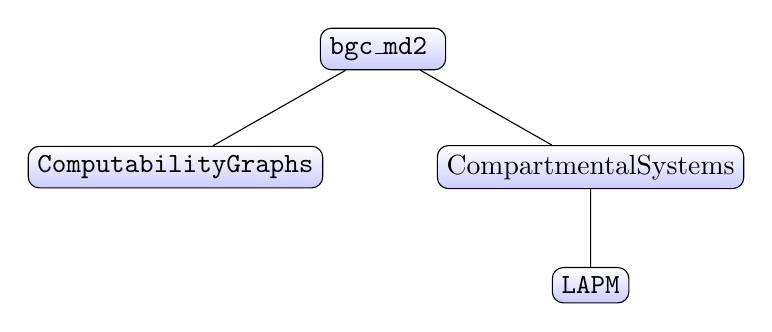
\begin{tikzpicture}[sibling distance=15em,
  every node/.style = {shape=rectangle, rounded corners,
    draw, align=center,
    top color=white, bottom color=blue!20}]]
    \node {
    	\texttt{bgc\_md2}
    }
    child { node {\texttt{ComputabilityGraphs}} }
	child { node[sibling distance=5em]{CompartmentalSystems}
	child { node (LAPM){\texttt{LAPM}} }
	%child [level distance=10em]{ node [style ={top color=white,bottom color=black!10}](SymPy){\texttt{SymPy}} }
	%child [level distance=10em]{ node [style ={top color=white,bottom color=black!10}](SymPy){\texttt{nupy}} }
   };
	%\draw[->] (LAPM) -- (SymPy); 
\end{tikzpicture}
}

  \note{
  \begin{enumerate}
    \item
    The graph computation is outsourced into our package \texttt{ComputabilityGraphs} 
    \item
	    Many of the advanced diagnostic variables (age and transittime distributions) are computed using our other packages \texttt{LAPM} and \texttt{CompartmentalSystems} for which \texttt{bgc\_md2} acts as interface.
  \end{enumerate}
}
\end{frame}
%\section{Applications}
%%%%%%%%%%%%%%%%%%%%%%%%%%%%%%%%%%%%%%%%%%%%%%%%%%%%%%%%%%%%%%%%%
\begin{frame}
  \frametitle{Example computation via \texttt{CompartmentalSystems}}
	\begin{figure}
	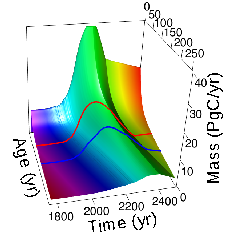
\includegraphics[height=0.5\textheight]{atmosphere_nonlinear.pdf}
		\caption{age distribuition of a pool as function of time}
	\end{figure}
  {\tiny
	\begin{thebibliography}{}
	\bibitem[Metzler, Müller, Sierra, 2018]{Metzler2018PNAS}
	Metzler, H., M{\"u}ller, M., and Sierra, C. (2018).
	\newblock Transit-time and age distributions for nonlinear time-dependent
	  compartmental systems.
	\newblock {\em Proceedings of the National Academy of Sciences}, 115:201705296.
	\end{thebibliography}
  }
\end{frame}
%%%%%%%%%%%%%%%%%%%%%%%%%%%%%%%%%%%%%%%%%%%%%%%%%%%%%%%%%%%%%%%%%
\mysection{Links}\label{links}
\begin{frame}
	\frametitle{Links}
  \begin{itemize}
    \item
      The README of the package on github (wiht installation instructions):
      \url{https://github.com/MPIBGC-TEE/bgc_md2}
    \item
      \url{https://mybinder.org/v2/gh/MPIBGC-TEE/bgc_md2/binder}
      binder for testing some 
      tutorials (jupyter notebooks) for the creation of new models or a model comparison
      No istallation neccessary.
  \end{itemize}
\end{frame}

\end{document}
